\documentclass[11pt]{article}
\usepackage[a4paper,margin=1in]{geometry}
\usepackage{amsmath,amssymb,amsthm}
\usepackage{graphicx}
\usepackage[hidelinks]{hyperref}

\newtheorem{theorem}{Theorem}
\newtheorem{lemma}{Lemma}
\newtheorem{corollary}{Corollary}
\newtheorem{remark}{Remark}

\DeclareMathOperator{\Stab}{Stab}

\title{Torsion Collapse for Noncommutative Cotlar Symbols}
\author{Automatic math-discovery packet}
\date{July 3, 2026}

\begin{document}
\maketitle

\section*{Source question}

The source paper is Adrian M. Gonzalez-Perez, Javier Parcet, and Runlian Xia,
\emph{Noncommutative Cotlar identities for groups acting on tree-like
structures}, arXiv:2209.05298. The paper proves that, for a discrete group
and \(G_0=\{e\}\), the noncommutative Cotlar identity for a Fourier multiplier
is equivalent to the closed formula
\begin{equation}
  \label{eq:cotlar}
  \bigl(m(g^{-1})-m(h)\bigr)\bigl(m(gh)-m(g)\bigr)=0,
  \qquad g\ne e,\ h\in G.
\end{equation}

After proving that UAC-space models produce such symbols, the source asks
whether there are Cotlar symbols that do not arise from the UAC models, or
whether a reverse construction is always possible.

\begin{figure}[h]
\centering
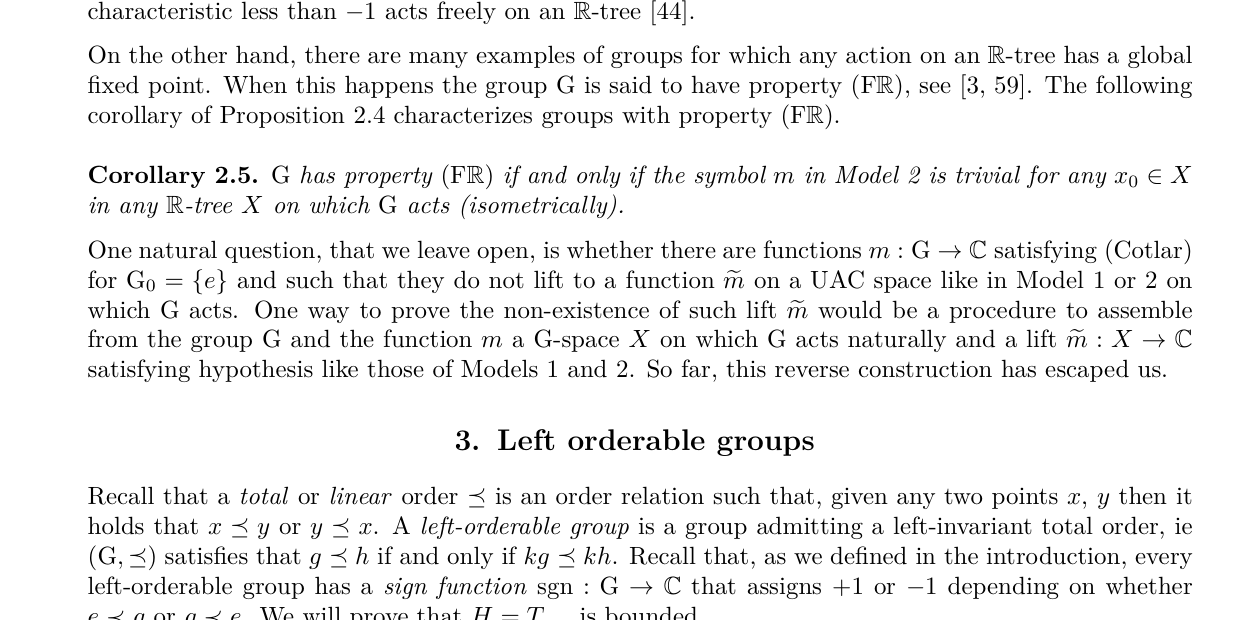
\includegraphics[width=\textwidth]{figures/reverse_uac_question_page21_crop.png}
\caption{The source's reverse-UAC question, on page 21 of the arXiv PDF.}
\end{figure}

\section*{Packet claim}

This packet proves a torsion obstruction. If \(G\) is a torsion group, then
\eqref{eq:cotlar} forces \(m\) to be constant away from the identity. Thus a
nontrivial counterexample to the reverse-UAC question cannot live on a torsion
group. The remaining constant-off-identity symbols are geometrically
uninteresting: they lift to Model 1 on a regular star tree.

\section*{Proof intuition}

The Cotlar formula is very rigid on finite cycles. If \(a\) has finite order
and \(m(a)\ne m(a^{-1})\), then applying \eqref{eq:cotlar} repeatedly with
\(g=a\) walks around the cyclic subgroup and forces every negative power of
\(a\) to have the value \(m(a^{-1})\), eventually including \(a\) itself, a
contradiction. Thus finite-order elements have the same value as their
inverses.

Now suppose two torsion elements \(a,b\ne e\) have different values. Applying
\eqref{eq:cotlar} to \(g=a\), \(h=a^{-1}b\) forces \(a^{-1}b\) to have the
same value as \(a\). Applying it to \(g=b\), \(h=b^{-1}a\) forces
\((a^{-1}b)^{-1}\) to have the same value as \(b\). Since \(a^{-1}b\) also has
finite order, inverse-symmetry gives a contradiction.

\section*{Main theorem}

\begin{lemma}[finite-order inverse symmetry]
\label{lem:inverse}
Let \(G\) be a group and let \(m:G\to\mathbb C\) satisfy
\eqref{eq:cotlar}. If \(a\in G\setminus\{e\}\) has finite order, then
\[
  m(a)=m(a^{-1}).
\]
\end{lemma}

\begin{proof}
If \(a^2=e\), the assertion is immediate. Assume that the order of \(a\) is
\(q\ge 3\), and suppose for contradiction that \(m(a)\ne m(a^{-1})\).
We prove by induction that
\[
  m(a^{-j})=m(a^{-1}) \qquad (1\le j\le q-1).
\]
The case \(j=1\) is tautological. Suppose the claim holds for some
\(1\le j\le q-2\). Apply \eqref{eq:cotlar} with \(g=a\) and
\(h=a^{-(j+1)}\). Since \(gh=a^{-j}\), we get
\[
  \bigl(m(a^{-1})-m(a^{-(j+1)})\bigr)
  \bigl(m(a^{-j})-m(a)\bigr)=0.
\]
By the induction hypothesis and by \(m(a^{-1})\ne m(a)\), the second factor
is nonzero. Hence \(m(a^{-(j+1)})=m(a^{-1})\).
Taking \(j=q-1\) gives
\[
  m(a)=m(a^{-(q-1)})=m(a^{-1}),
\]
contradicting the assumption. Therefore \(m(a)=m(a^{-1})\).
\end{proof}

\begin{theorem}[torsion Cotlar collapse]
\label{thm:torsion}
Let \(G\) be a torsion group and let \(m:G\to\mathbb C\) satisfy
\eqref{eq:cotlar}. Then there is a scalar \(\alpha\in\mathbb C\) such that
\[
  m(g)=\alpha \qquad \text{for every } g\in G\setminus\{e\}.
\]
\end{theorem}

\begin{proof}
Assume that there are \(a,b\in G\setminus\{e\}\) with \(m(a)\ne m(b)\).
Then \(a\ne b\), so \(c=a^{-1}b\ne e\). Since \(G\) is torsion, \(a\), \(b\),
and \(c\) all have finite order.

Apply \eqref{eq:cotlar} with \(g=a\) and \(h=c=a^{-1}b\). Since \(gh=b\), we
obtain
\[
  \bigl(m(a^{-1})-m(c)\bigr)\bigl(m(b)-m(a)\bigr)=0.
\]
The second factor is nonzero, so Lemma \ref{lem:inverse} gives
\[
  m(c)=m(a^{-1})=m(a).
\]
Similarly, applying \eqref{eq:cotlar} with \(g=b\) and
\(h=b^{-1}a=c^{-1}\) gives
\[
  m(c^{-1})=m(b^{-1})=m(b).
\]
But \(c\) has finite order, so Lemma \ref{lem:inverse} also gives
\[
  m(c)=m(c^{-1}).
\]
Thus \(m(a)=m(b)\), a contradiction. Hence all nonidentity elements have the
same value.
\end{proof}

\section*{Consequence for the reverse-UAC question}

\begin{corollary}
No torsion group can provide a nonconstant Cotlar symbol for the reverse-UAC
question with \(G_0=\{e\}\). More precisely, every Cotlar symbol on a torsion
group is constant off the identity and has a Model 1 lift on a UAC space.
\end{corollary}

\begin{proof}
The first assertion is Theorem \ref{thm:torsion}. It remains to describe the
lift for a symbol with
\[
  m(e)=\beta,\qquad m(g)=\alpha\quad(g\ne e).
\]
Let \(X\) be the star tree with one branch \([0,1]_r\) for each \(r\in G\),
all glued at \(0\). Let \(G\) act by permuting branches:
\[
  k\cdot (t,r)=(t,kr).
\]
Choose \(x_0=(1,e)\). Then \(\Stab(x_0)=\{e\}\), and \(X\setminus\{x_0\}\)
is arcwise connected. Define
\[
  \widetilde m(x_0)=\beta,\qquad
  \widetilde m(x)=\alpha\quad(x\ne x_0).
\]
This function is constant along arcs in \(X\setminus\{x_0\}\) and is invariant
under the stabilizer of \(x_0\). Therefore it is a Model 1 lift, and
\[
  \widetilde m(g\cdot x_0)=m(g)
\]
for every \(g\in G\).
\end{proof}

\section*{Scope and limitations}

This is not a full solution of the reverse-UAC problem. It shows that a
nontrivial counterexample must use group elements of infinite order. More
locally, the proof shows that if \(a,b,a^{-1}b\) all have finite order, then
any Cotlar symbol satisfying \eqref{eq:cotlar} must have \(m(a)=m(b)\).

The theorem also does not address the convex-hull problem for Cotlar-type
multipliers or the endpoint-space problem from the same source paper.

\section*{Novelty and search status}

This packet was produced as a direct attack on the source question. Bounded
searches were run for phrases including ``Cotlar torsion group constant
Fourier multiplier'', ``Noncommutative Cotlar identities torsion'', and
``2209.05298 torsion Cotlar'', and for the source title together with
``reverse construction'' and ``UAC''. The searches found the source arXiv page
but no prior statement of the torsion-collapse lemma. This is a partial
novelty check only; the result should be reviewed as a short algebraic
observation adjacent to the source question.

\section*{Computational sanity check}

The script \texttt{code/finite\_cotlar\_search.py} exhausts all three-color
equality patterns on a few small finite groups, including cyclic groups,
dihedral groups, \(S_3\), and elementary \(2\)-groups of ranks \(2\) and \(3\).
It finds no nonconstant-off-identity patterns. The proof above does not rely
on this computation.

\section*{Verification notes}

The proof uses only the closed Cotlar formula \eqref{eq:cotlar}. The induction
in Lemma \ref{lem:inverse} is the only cyclic argument: once
\(m(a^{-j})=m(a^{-1})\ne m(a)\), the Cotlar formula with
\(g=a\), \(h=a^{-(j+1)}\) forces the next negative power to have the same
value. Theorem \ref{thm:torsion} then uses the finite order of \(a^{-1}b\);
this is exactly where the torsion hypothesis enters.

\section*{Human-review recommendation}

Review as a likely valid partial result. The key checks are Lemma
\ref{lem:inverse}, the use of \(c=a^{-1}b\) in Theorem \ref{thm:torsion}, and
the claim that the regular-star tree gives a legitimate Model 1 lift for the
constant-off-identity case.

\begin{thebibliography}{9}

\bibitem{GPX}
A. M. Gonzalez-Perez, J. Parcet, and R. Xia,
\emph{Noncommutative Cotlar identities for groups acting on tree-like
structures}, arXiv:2209.05298.

\end{thebibliography}

\end{document}
